\graphicspath{{./Chapters/CH3/Pictures/}}
\let\cleardoublepage\clearpage

\section{Overview and Categorization}
\subsection{Overview}
\label{subsec:mpc-overview}

Model predictive control (MPC) brings a simple promise to power electronics: decide the next switching action by looking one step into the future and choosing the option that best serves the objectives. Unlike classical controllers that shape dynamics indirectly through gains and bandwidths, MPC works with an explicit model of the converter–machine pair and a concrete statement of what “good” means—tracking accuracy, modest switching activity, bounded voltages and currents, and respect for hardware limits. In a drive inverter these choices must be made at microsecond time scales; the plant is hybrid (continuous currents driven by discrete switch positions), the actuation is constrained (finite switching states and a limited voltage polygon), and nonidealities such as dead time and device drops lightly bend the physics. MPC fits this geometry naturally.

At each sampling instant the controller predicts what the electrical variables will do under a set of candidate actions, evaluates a cost for each candidate, and applies the one with the smallest cost. When the candidate set is the finite collection of inverter switching states, the controller decides which vector to apply next; when the decision is a continuous voltage or duty vector, the controller computes an optimal value and then realizes it with modulation. In both cases the essential ingredients are the same: a discrete-time prediction model, a cost function that encodes the priorities of the application, explicit constraints, and an implementation that closes the loop deterministically within the sampling budget. This chapter organizes those ingredients for power-electronics systems and sets the stage for the motor-drive controller designed later.

\subsection{Categorization of MPC Approaches}

There are two principal MPC flavors in power converters.
FCS-MPC treats the inverter as a device with a small catalogue of admissible switching vectors. The controller evaluates all admissible vectors over a short horizon—often a single step—and chooses the one that best advances the target. The advantages are conceptual simplicity, direct handling of discrete actuation, and constant computational cost; the tradeoff is higher current ripple unless special measures (virtual vectors, horizon extension, or switching penalties) are employed.
Continuous-control-set MPC optimizes a continuous voltage (or duty) command using the prediction model and then realizes that command with a modulator such as space-vector PWM. The benefit is low ripple and direct access to classical constraints on voltages and currents; the tradeoff is a small layer of modulation logic and, in general, slightly higher computational burden.

In motor drives, the most common targets are the stator currents or the electromagnetic torque; flux and power are also used in special cases. Current-tracking MPC provides a natural inner loop; torque-tracking MPC absorbs the current-to-torque mapping into the prediction model and cost, which can simplify the outer speed loop. DC-link voltage or grid current tracking dominate in rectifiers and active front ends.

Most drive applications use a one-step horizon with delay compensation, which aligns with tight sampling budgets and yields dead-beat-like behavior. Two-step horizons can reduce ripple or incorporate switching frequency penalties more gracefully. In all cases, the timing model—sample, compute, and apply—must be explicit so that the prediction lands at the instant when the action actually appears at the machine terminals.

Linear models in stationary or synchronous frames are customary and sufficient for fast inner loops. Nonidealities (dead time, device drops, computation and ADC delays, saturation of the voltage vector) are often included through additive biases, effective voltage reduction, or explicit constraints in the cost. Where parameter drift is expected (for example, resistance with temperature), adaptive updates or observer-based estimates can be incorporated without changing the controller’s structure.


The cost function is the language in which priorities are expressed. A typical current-tracking term measures the error at the prediction instant; a switching-effort term discourages unnecessary transitions; soft constraints penalize excursions beyond the linear modulation region or current limits, while hard constraints clip decisions that are physically unreachable. Weighting can be normalized to physical units (volts, amperes, radians per second) to make tuning interpretable and portable across operating points.


In direct MPC the selected switching state is applied immediately by the gate driver. In M2PC a continuous reference voltage or duty vector is passed to an SVM block, which generates duty ratios while preserving the average voltage commanded by the optimizer. Both realizations can be embedded in the same framework; the choice is guided by ripple, efficiency, electromagnetic compatibility, and processor headroom.


This thesis adopts a formulation that is tailored to motor drives and their inverter non-idealities. The controller is expressed in the synchronous frame with a short prediction horizon, uses an average inverter model driven by space-vector duty cycles, and encodes both tracking accuracy and inverter limits in a compact cost. Nonidealities are represented within the prediction and decision layers rather than treated post-hoc, allowing the controller to anticipate and mitigate their effect. Subsequent sections develop the prediction model, the cost terms, and the real-time realization that make this possible.


% ==========================================================
% Section: Discrete-Time Models for Power Converters
% Requires: \usepackage{amsmath}
% ==========================================================


% ==========================================================
% Section: Finite-Control-Set MPC for a Two-Level Inverter
% Requires: \usepackage{amsmath,booktabs}
% ==========================================================

% ==========================================================
% Section: Finite-Control-Set MPC for a Two-Level Inverter
% (Detailed and simplified narrative, step-by-step)
% Requires: \usepackage{amsmath}
% ==========================================================

% ==========================================================
% Section: Finite-Control-Set MPC for a Two-Level Inverter
% (Explained as a method, step-by-step)
% Requires: \usepackage{amsmath}
% ==========================================================

% ==========================================================
% Finite-Control-Set MPC (with in-text figure references)
% Requires: \usepackage{amsmath,graphicx}
% ==========================================================

% -------- Figures placed near the discussion; LaTeX will float them --------

\section{Finite-Control-Set MPC for a Two-Level Inverter}
\label{sec:fcsmpc}

\subsection{Methodology}
Every sampling period, the inverter must output exactly one switching state. The idea of FCS–MPC is simple: we list the few admissible states, we predict what the motor currents would look like if we applied each one, we score those predictions with a small cost, and we choose the state with the lowest score. No duty computation and no PWM are required in the pure form as shown in Figure~\ref{fig:fcs-diagram}.

\begin{figure}[H]
  \centering
  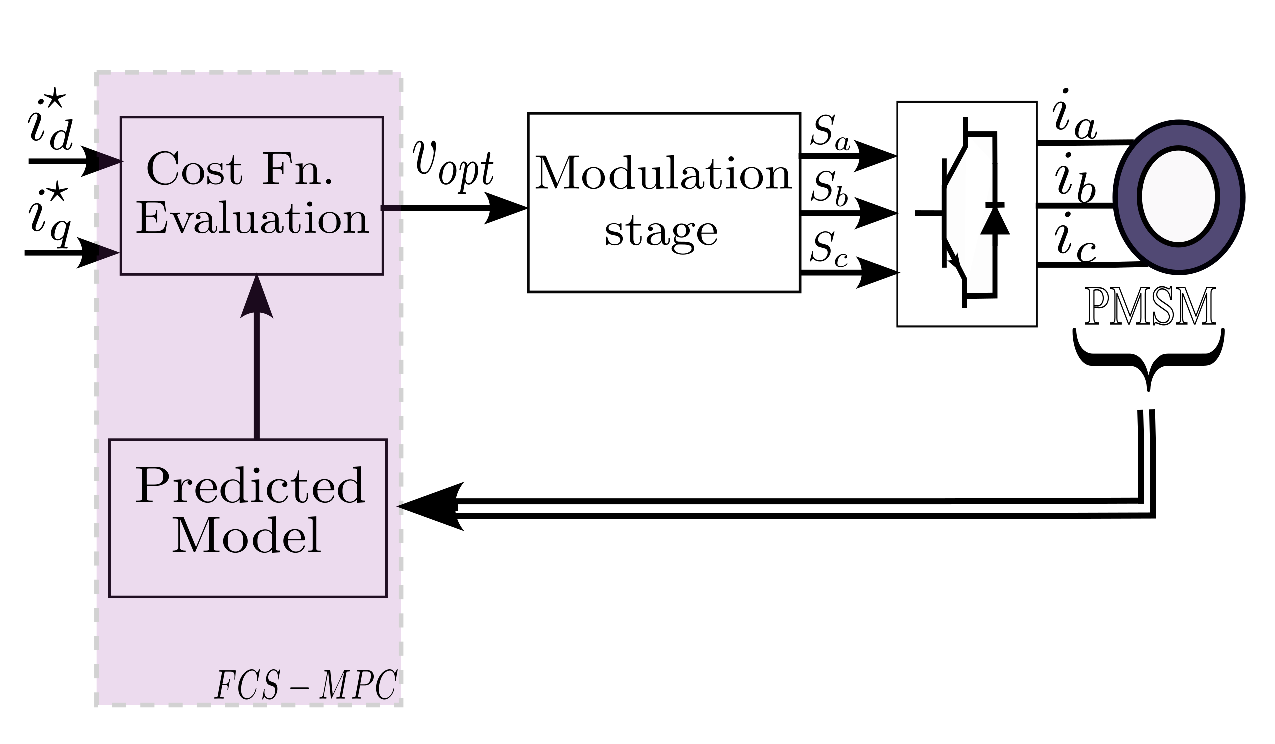
\includegraphics[width=\linewidth]{FCS}
  \caption{Control schematic for the FCS–MPC drive.}
  \label{fig:fcs-diagram}
\end{figure}


At the start of the control loop we have the measured/estimated currents, the electrical angle and speed, the DC-bus voltage, and the switching state that is currently being applied (from the previous decision). We also have the current references that we want to track at the prediction instant.
\begin{equation}
\label{eq:fcs-known}
\mathbf i[k]=\begin{bmatrix}i_d[k]\\ i_q[k]\end{bmatrix},\quad
\theta_e[k],\ \omega_e[k],\ V_{\mathrm{dc}}[k],\ \mathbf S[k{-}1], \mathbf i^{\ast}[k{+}2]
\end{equation}


Each inverter leg is either low ($0$) or high ($1$):
\begin{equation}
\label{eq:fcs-S}
\mathbf S=\begin{bmatrix}S_a\\ S_b\\ S_c\end{bmatrix}\in\{0,1\}^3 .
\end{equation}
There are six active states and two zero states as shown in Figure \ref{fig:InverterStates}. We usually test the six active states and optionally the zeros at very low speed or during limiting.

\begin{figure}[h]
	\centering
	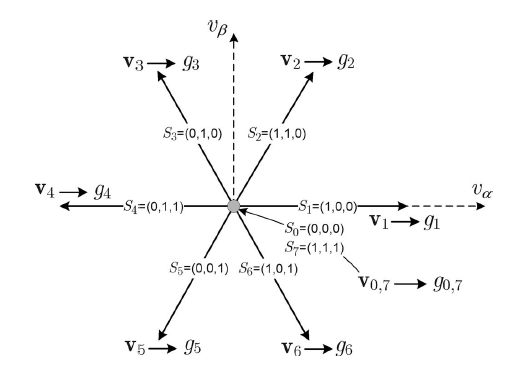
\includegraphics[width=\textwidth]{./InverterStates}
	\caption{Two Level Inverter Switching States}
	\label{fig:InverterStates}
\end{figure}

Given a candidate $\mathbf S_{i}$, we compute its stationary-frame voltages with two short formulas. First remove common mode and apply the Clarke map (written here in closed form):
\begin{equation}
\label{eq:fcs-valpha}
v_\alpha(\mathbf S_{i}) \;=\; V_{\mathrm{dc}}\!\left(\tfrac{2}{3}S^{i}_a-\tfrac{1}{3}S^{i}_b-\tfrac{1}{3}S^{i}_c\right),
\end{equation}
\begin{equation}
\label{eq:fcs-vbeta}
v_\beta(\mathbf S_{i}) \;=\; \frac{V_{\mathrm{dc}}}{\sqrt{3}}\,(S^{i}_b-S^{i}_c).
\end{equation}
We then rotate to the synchronous frame at the current electrical angle:
\begin{equation}
\label{eq:fcs-vdq}
\begin{bmatrix} v_d(\mathbf S_{i}) \\[2pt] v_q(\mathbf S_{i}) \end{bmatrix}
=
\begin{bmatrix}
\cos\theta_e[k] & \sin\theta_e[k]\\[2pt]
-\sin\theta_e[k] & \cos\theta_e[k]
\end{bmatrix}
\begin{bmatrix} v_\alpha(\mathbf S_{i}) \\[2pt] v_\beta(\mathbf S_{i}) \end{bmatrix}.
\end{equation}

We use the SPMSM electrical model in $dq$ and a one-step (or two-step) forward–Euler update. The continuous-time model is
\begin{equation}
\label{eq:fcs-ct}
\begin{bmatrix}\dot i_d\\[2pt]\dot i_q\end{bmatrix}
=
\frac{1}{L_s}
\begin{bmatrix}
- R_s & \ \ \ \omega_e L_s\\[2pt]
- \omega_e L_s & - R_s
\end{bmatrix}
\begin{bmatrix} i_d\\[2pt] i_q\end{bmatrix}
+
\frac{1}{L_s}\begin{bmatrix} v_d\\[2pt] v_q\end{bmatrix}
+
\frac{1}{L_s}\begin{bmatrix} 0\\[2pt] -\omega_e \lambda_f\end{bmatrix}.
\end{equation}
Freezing coefficients at time $k$, the one-step prediction under $\mathbf S$ is
\begin{equation}
\label{eq:fcs-euler}
\hat{\mathbf i}[k{+}1 ]
= \mathbf i[k]
+\frac{T_s}{L_s}\!\left(
\begin{bmatrix}
- R_s & \ \ \ \omega_e[k] L_s\\[2pt]
- \omega_e[k] L_s & - R_s
\end{bmatrix}\!\mathbf i[k]
+\begin{bmatrix} v_d(\mathbf S[k-1])\\[2pt] v_q(\mathbf S[k-1])\end{bmatrix}
+\begin{bmatrix} 0\\[2pt] -\omega_e[k]\lambda_f\end{bmatrix}
\right)\!.
\end{equation}
We first advance one step using the \emph{previous} state, then advance a second step with the \emph{candidate} state:
\begin{equation}
\label{eq:fcs-delay-1}
\hat{\mathbf i}[k{+}1]=\text{\eqref{eq:fcs-euler} evaluated with }\mathbf S[k{-}1],
\end{equation}
\begin{equation}
\label{eq:fcs-delay-2}
\hat{\mathbf i}^{i}[k{+}2]=\hat{\mathbf i}[k{+}1]
+\frac{T_s}{L_s}\!\left(
\begin{bmatrix}
- R_s & \ \ \ \omega_e[k] L_s\\[2pt]
- \omega_e[k] L_s & - R_s
\end{bmatrix}\!\hat{\mathbf i}[k{+}1]
+\begin{bmatrix} v_d(\mathbf S_{i})\\[2pt] v_q(\mathbf S_{i})\end{bmatrix}
+\begin{bmatrix} 0\\[2pt] -\omega_e[k]\lambda_f\end{bmatrix}
\right)\!.
\end{equation}
We compare \eqref{eq:fcs-euler} to a $k{+}1$ reference when there is no delay, and \eqref{eq:fcs-delay-2} to a $k{+}2$ reference when there is a one-sample delay.


The cost has a tracking term (normalized so tuning is consistent) and, optionally, a switching penalty to limit toggles. The tracking term is
\begin{equation}
\label{eq:fcs-Ji}
J_i(\mathbf S_{i}) \;=\; \big\| \mathbf W_i \big(\mathbf i^{\ast}[k{+}2]-\hat{\mathbf i^{i}}[k{+}2 ]\big) \big\|_2^2,
\end{equation}
with a simple diagonal normalizer
\begin{equation}
\label{eq:fcs-Wi}
\mathbf W_i=\mathrm{diag}\!\Big(\frac{1}{I_d^{\mathrm n}},\,\frac{1}{I_q^{\mathrm n}}\Big).
\end{equation}
The switching effort is penalized by counting how many legs would change:
\begin{equation}
\label{eq:fcs-Jdu}
J_{\Delta u}(\mathbf S_{i})=\lambda_{\Delta u}\,\big\|\mathbf S_{i}[k]-\mathbf S[k-1]\big\|_1,
\end{equation}
and the total cost is
\begin{equation}
\label{eq:fcs-J}
J_{i}=J_i(\mathbf S_{i})+J_{\Delta u}(\mathbf S_{i}).
\end{equation}

We choose the state with the smallest cost and hand it to the gate driver:
\begin{equation}
\label{eq:fcs-argmin}
\mathbf S^\star[k] \;=\; \arg\min_{\mathbf S\in\{0,1\}^3} J_{i}.
\end{equation}


\subsection{Algorithm Summary}
% FCS-MPCC in dq-frame — Summarized Steps (paste-ready)
\begin{enumerate}
  \item Define controller data: \(T_s\), machine/inverter parameters, limits, weights, and delay/dead-time compensation settings.
  \item Acquire signals each \(T_s\): \(i_d,i_q\), \(\theta_e,\omega_e\), \(V_{dc}\) (and any estimator outputs).
  \item Set references from outer loops: \(i_d^\star, i_q^\star\); apply saturation and rate limits.
  \item Enumerate feasible inverter switching states (e.g., 8 for a 2-level VSI).
  \item For each candidate state: compute its stator voltage vector, apply dead-time/device-drop compensation, and transform to the \(dq\) frame using \(\theta_e(k)\).
  \item Predict next-step \(i_d,i_q\) for each candidate using the discrete PMSM model (include one-step delay compensation; optionally use a two-step horizon).
  \item Evaluate a cost for each candidate:
        primary term = current-tracking error w.r.t. \(i_d^\star,i_q^\star\), and the switching effort;.
  \item Enforce constraints and discard infeasible candidates (current/voltage/thermal/speed).
  \item Select the candidate with minimum cost..
  \item Apply the selected switching state for the next control period.
  \item Update observers/estimators and any parameter adaptation; refresh \(\theta_e,\omega_e\); repeat each \(T_s\).
\end{enumerate}


\subsection{Modeling and Simulations}
This section validates the complete drive model and controllers through a focused suite of studies: (i) steady-state operation to verify ripple, losses, and harmonic content; (ii) low-speed operation to probe back-EMF limits and non-idealities; (iii)  dynamic performance under speed/current steps; (iv) parameter variation to gauge robustness against model mismatch; and (v) load variation to assess torque disturbance rejection.
\subsubsection{Steady State Operation}
At 1000 rpm (50\% rated) and 50\% rated load (\(1.75~\mathrm{N\,m}\)), the finite–control–set MPC produces the correct average torque but exhibits a phase–current THD of 8\% (see Fig.~\ref{fig:FCSIdeal_1000rpm_med}). This is characteristic of FCS applying a single vector per sample and frequently toggling between adjacent active vectors, which creates a staircase voltage, larger current ripple, and visible torque pulsations—even in the absence of non-idealities—yielding only moderate steady-state quality.

% Requires in preamble:
% \usepackage{graphicx}
% \usepackage{subcaption}

\begin{figure}[H]
  \centering
  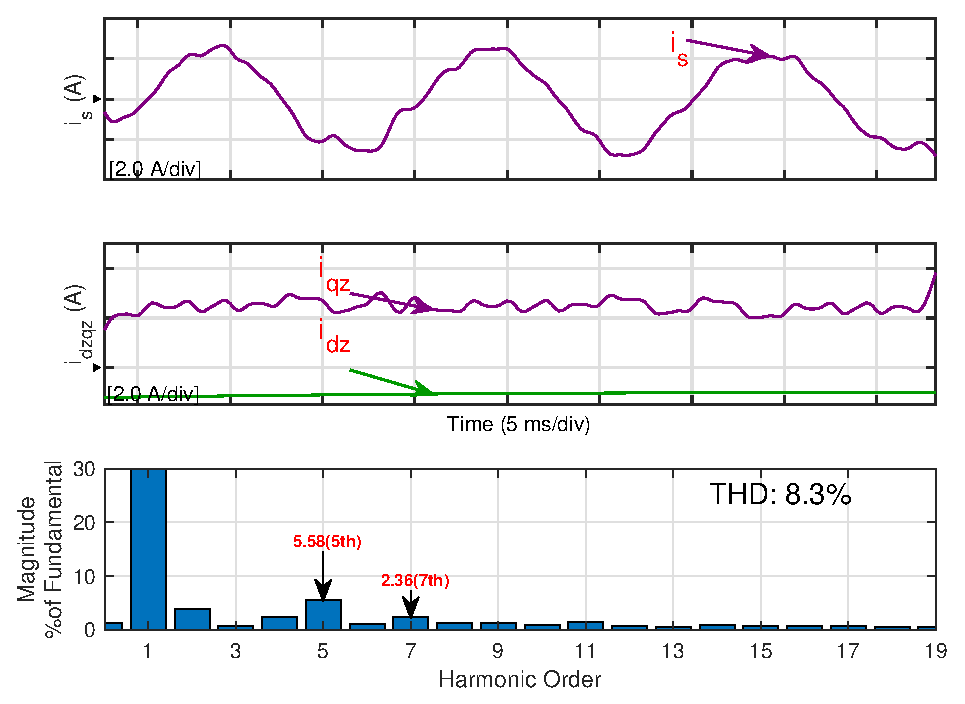
\includegraphics[width=0.7\linewidth]{./FCSMidSpeedMidLoadSteadyState}
  \caption{FCS–MPC steady state at 50\% rated speed (1000 rpm) and 50\% rated load (\(1.75~\mathrm{N\,m}\), ideal model). Panels show (a) phase current, (b) \(dq\) currents, and (c) THD (\(8\%\)).}
  \label{fig:FCSIdeal_1000rpm_med}
\end{figure}

\subsubsection{Low Speed Operation}
At 100 rpm (5\% rated) with an ideal inverter, the FCS controller applies a single active vector per sample; at \emph{low load} (10\% rated, \(0.3~\mathrm{N\,m}\)) the commanded stator voltage is tiny relative to the nearest active vector, so hexagon quantization is coarse and the staircase phase voltage yields 32\% THD (see Fig.~\ref{fig:FCSIdeal_100rpm_low}). At \emph{rated load} (\(3.5~\mathrm{N\,m}\)), the average voltage grows, the relative vector mismatch shrinks, and THD drops to 4\% (see Fig.~\ref{fig:FCSIdeal_100rpm_high}). Even under ideal conditions this remains above the PI baseline at 100 rpm (\(\mathbf{1.3\%}\) THD; Fig.~\ref{fig:PIIdeal_100rpm}), highlighting FCS’s intrinsic steady-state penalty at low-voltage operating points despite correct average torque.

\begin{figure}[H]
  \centering
  \begin{subfigure}{0.485\textwidth}
    \centering
    % Replace with your exported plot/image
    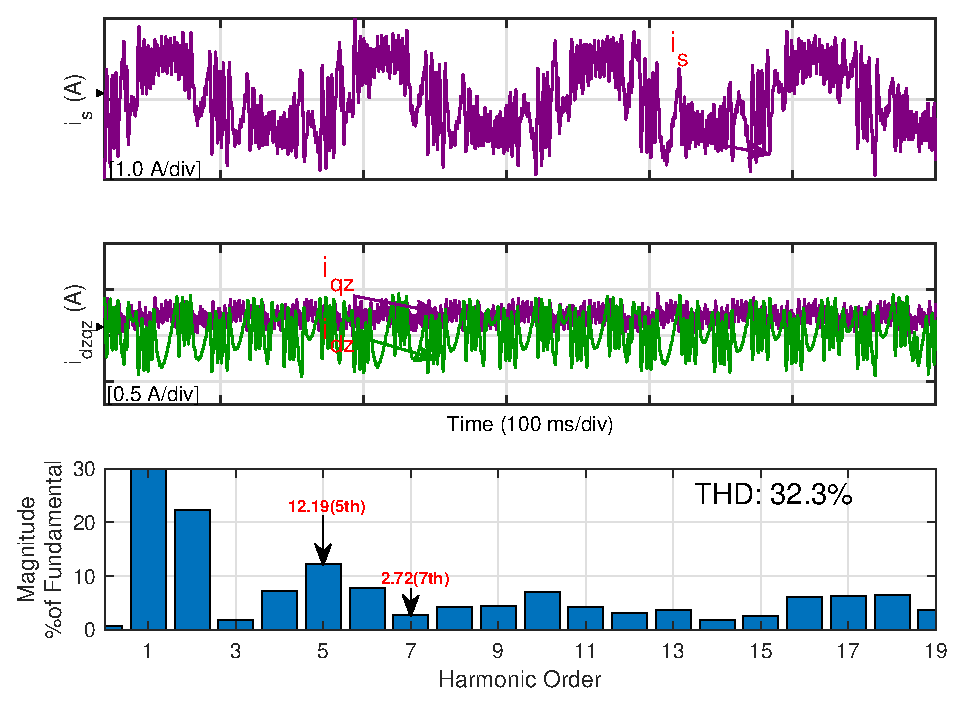
\includegraphics[width=\linewidth]{./FCSSteadyStateLowLoad100Rpm}
    \caption{Low load: \(T=0.3~\mathrm{N\,m}\), THD \(=32\%\).}
    \label{fig:FCSIdeal_100rpm_low}
  \end{subfigure}\hfill
  \begin{subfigure}{0.485\textwidth}
    \centering
    % Replace with your exported plot/image
    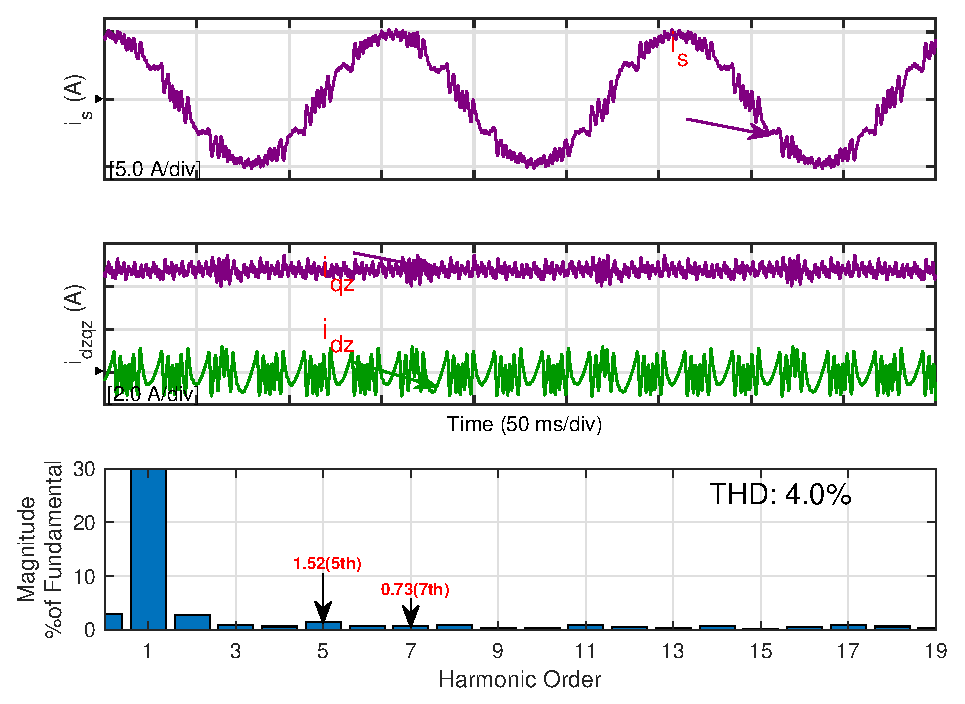
\includegraphics[width=\linewidth]{./FCSSteadyStateHighLoad100Rpm}
    \caption{Rated load: \(T=3.5~\mathrm{N\,m}\), THD \(=4\%\).}
    \label{fig:FCSIdeal_100rpm_high}
  \end{subfigure}
  \caption{FCS–MPC at low speed (100 rpm, ideal model). Each panel reports phase current, \(i_{dq}\), and THD; the low–load case shows coarse vector quantization and high ripple, while the rated–load case exhibits reduced mismatch and lower THD.}
  \label{fig:FCSIdeal_100rpm}
\end{figure}

\subsubsection{Dynamic Performance}
With an ideal plant/inverter (no non-linearities or disturbances), the FCS controller tracks speed commands within the 10–50\% band (100~rpm \(\rightarrow\) 1000~rpm) at both load extremes without failure or steady-state deviation. At low load (\(0.3~\mathrm{N\,m}\)), Fig.~\ref{fig:FCSDyn_100to1000_low} shows correct tracking but overshoot \emph{exceeds} \(10\%\) and \(i_q\)/phase currents carry pronounced ripple; at rated load (\(3.5~\mathrm{N\,m}\)), Fig.~\ref{fig:FCSDyn_100to1000_rated} exhibits similar behavior with slightly slower damping. This stems from FCS’s single-vector actuation: during transients it toggles between adjacent vectors, producing a staircase voltage that amplifies current ripple and torque pulsations compared to the PI benchmark.
% Requires in preamble:
% \usepackage{graphicx}
% \usepackage{subcaption}

\begin{figure}[H]
  \centering
  % --- (a) Low load ---
  \begin{subfigure}{0.485\textwidth}
    \centering
    % Replace with your exported plot/image
    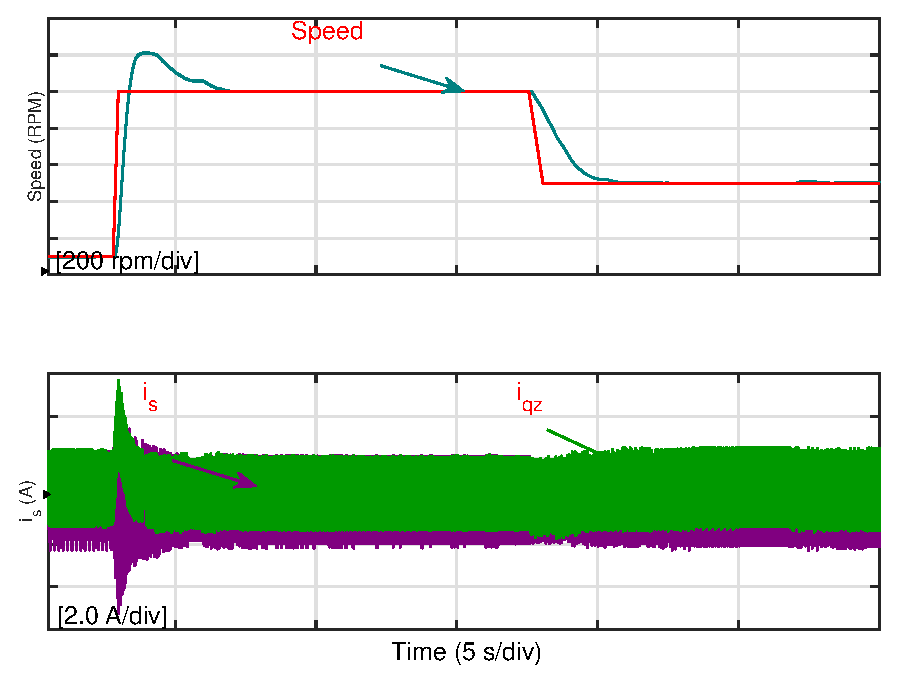
\includegraphics[width=\linewidth]{./FCSDynamicResponseLowLoad}
    \caption{Low load: \(T=0.3~\mathrm{N\,m}\). Overshoot \(>10\%\); pronounced \(i_q\)/phase-current ripple.}
    \label{fig:FCSDyn_100to1000_low}
  \end{subfigure}\hfill
  % --- (b) Rated load ---
  \begin{subfigure}{0.485\textwidth}
    \centering
    % Replace with your exported plot/image
    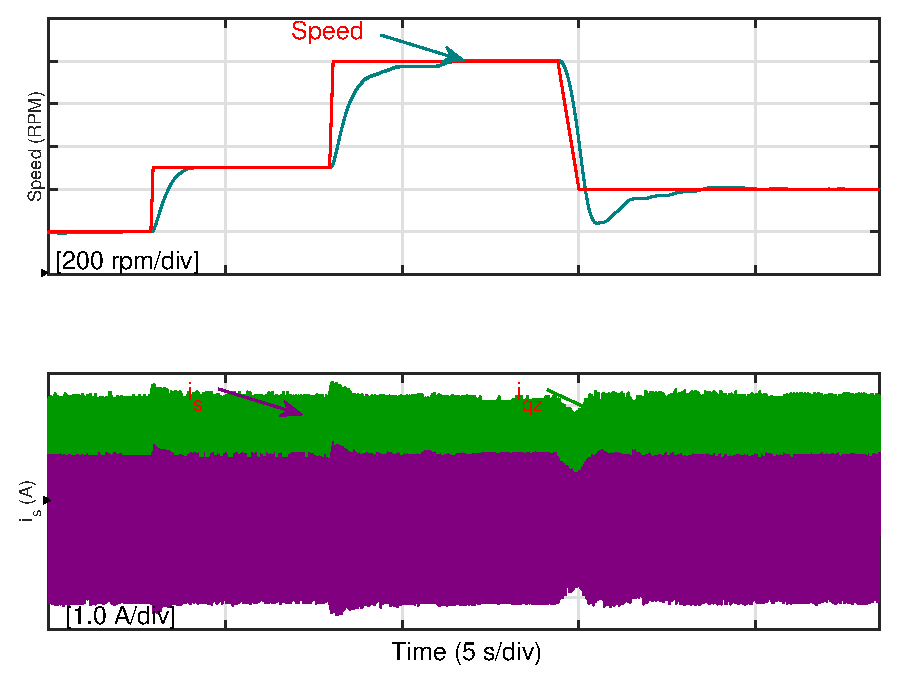
\includegraphics[width=\linewidth]{./FCSDynamicResponseHighLoad}
    \caption{Rated load: \(T=3.5~\mathrm{N\,m}\). Correct tracking, overshoot \(>10\%\); slightly slower damping.}
    \label{fig:FCSDyn_100to1000_rated}
  \end{subfigure}

  \caption{FCS–MPC dynamic response (ideal model) for speed changes within the \(10\%\!\to\!50\%\) rated band (100~rpm to 1000~rpm). Panels report command vs.\ speed, \(i_q\), and phase currents for (a) low load and (b) rated load.}
  \label{fig:FCSDyn_100to1000}
\end{figure}


\subsubsection{Parameter Variation}
To stress the prediction stage, the FCS controller was run with a deliberately biased internal model—stator resistance increased by \(+25\%\) and inductances decreased by \(25\%\)—while the plant and inverter remained ideal and the operating point was the worst case of 100 rpm (5\% rated). Under this mismatch the phase-current THD rose from \(\mathbf{32\%}\) (nominal model) to \(\mathbf{41\%}\). The degradation is expected: FCS ranks a single inverter vector per sample using one-step current predictions; errors in \(R_s\) and \(L\) bias those predictions, leading to suboptimal vector choices and coarser effective quantization on the hexagon. The result is amplified current harmonics and torque ripple—even without any non-idealities or disturbances—highlighting the sensitivity of FCS to prediction-model fidelity at low-voltage operating points.
% Requires in preamble:
% \usepackage{graphicx}

\begin{figure}[H]
  \centering
  % Replace with your exported composite plot (phase currents, dq currents, and THD)
  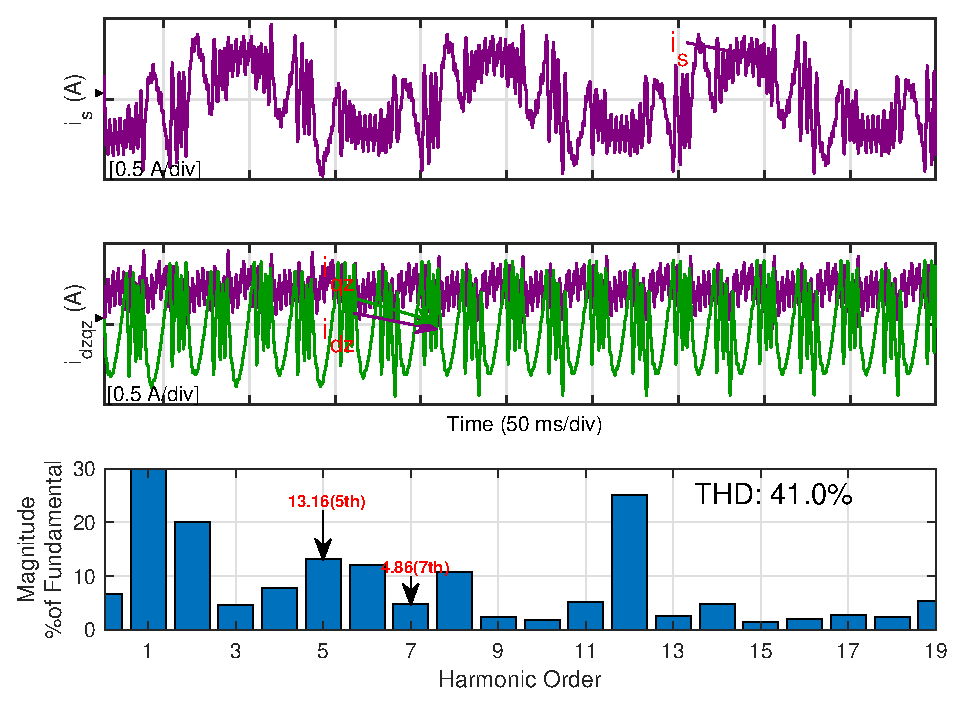
\includegraphics[width=0.7\linewidth]{./FCSParameterVariation}
  \caption{FCS–MPC parameter variation at low speed (100 rpm, ideal model). The prediction model uses \(R_s{+}25\%\) and \(L_{d,q}{-}25\%\). The composite plot shows (left) phase currents with enhanced ripple, (middle) \(d\)- and \(q\)-axis currents, and (right) THD comparison—rising from \(\mathbf{32\%}\) (nominal model) to \(\mathbf{41\%}\) (biased model) due to suboptimal vector selection from prediction errors.}
  \label{fig:FCSParamVariation}
\end{figure}

\subsubsection{Load Variation}
At 1000 rpm, the load torque was stepped from 10\% to 100\% of rated in 20\% increments, each plateau held to steady state. As shown in Fig.~\ref{fig:FCSLoadVariation}, the commanded speed is maintained without droop; Fig.~\ref{fig:FCSLoadVariation} shows \(i_q\) rising in clean steps to furnish the added torque; and Fig.~\ref{fig:FCSLoadVariation} reports the phase currents with the characteristic FCS staircase ripple—transients remain well damped, confirming robust regulation under load changes.

\begin{figure}[H]
  \centering
  % Replace with your exported composite plot that contains
  % (left) speed response, (middle) dq-currents, (right) phase currents
  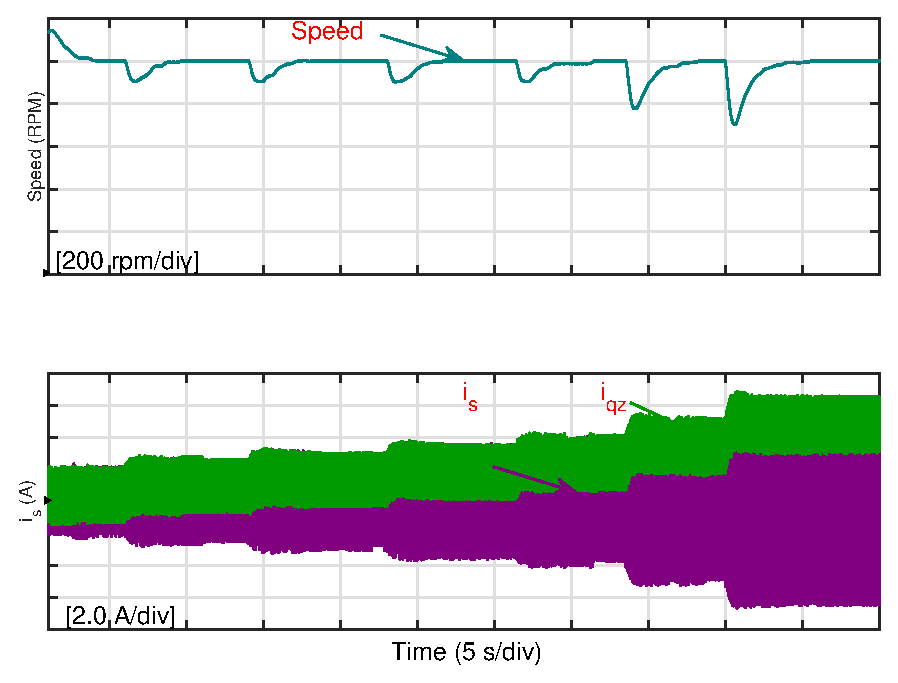
\includegraphics[width=0.6\linewidth]{./FCSLoadVariation}
  \caption{FCS–MPC under load variation at 50\% rated speed (1000 rpm, ideal model).
  The composite figure shows the speed response (measured), \(q\)-axis currents, and the phase currents during torque steps from 10\% to 100\% of rated in 20\% increments.}
  \label{fig:FCSLoadVariation}
\end{figure}

% ==========================================================
% Section: Continuous-Control-Set MPC (CCS-MPC) with Modulation
% Requires: \usepackage{amsmath,booktabs}
% ==========================================================

% ==========================================================
% Section: Modulated Model Predictive Control (MMPC) with SVM
% Requires: \usepackage{amsmath,graphicx}
% ==========================================================

% ==========================================================
% Section: Modulated Model Predictive Control (M2PC) with SVM
% (Forward–Euler discretization; detailed derivation)
% Requires: \usepackage{amsmath,graphicx}
% ==========================================================

% ==========================================================
% Modulated Model Predictive Control (Forward–Euler, story form)
% Requires: \usepackage{amsmath,graphicx}
% ==========================================================

\section{Modulated Model Predictive Control}
\label{sec:mmpc}

\subsection{Methodology}
The rationale for moving beyond FCS–MPC (Sec.~\ref{sec:fcsmpc}) is straightforward. Applying a single active vector per period makes the switching frequency state-dependent and pushes actuation to the hexagon edges, which increases current ripple, spreads the spectrum, and forces heuristic switching-penalty tuning. The modulated predictive controller adopted here preserves the same one-step, model-based “look ahead and choose” idea, but it optimizes a continuous average voltage that is realized by space–vector modulation (SVM). Practically, at each sampling instant we evaluate what would happen if each inverter vector were applied over the next period, select the two adjacent active vectors that best reduce the current error, and compute their dwell times (plus a zero vector) so that the average current error over the period is driven to zero. The outcome is a fixed switching frequency by construction, reduced ripple and acoustic noise, an explicit voltage-feasibility check, and a clean path to include non-idealities as effective voltage biases. In this work, the electrical prediction uses a Forward–Euler discretization for simplicity and deterministic real-time load.

\begin{figure}[H]
  \centering
  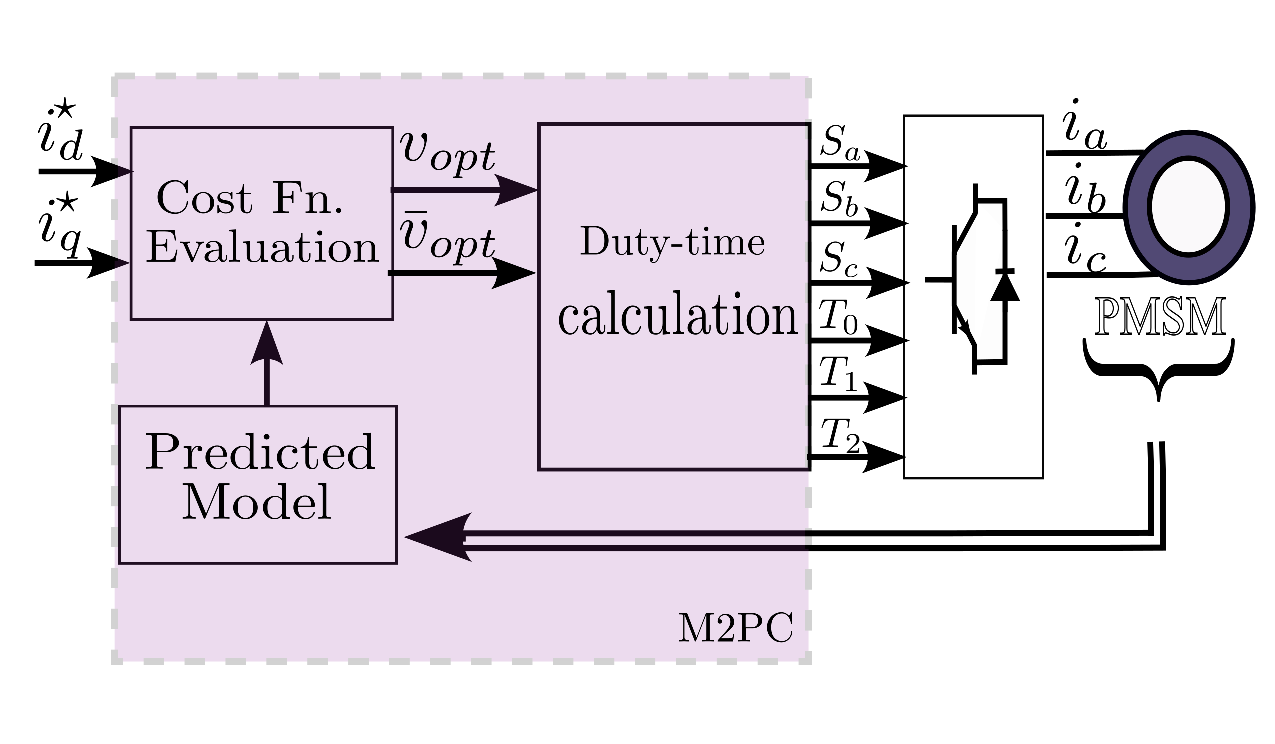
\includegraphics[width=\linewidth]{M2PC}
  \caption{Control schematic for the Modulated Model Predictive Controller Drive.}
  \label{fig:m2pc-diagram}
\end{figure}

The story begins by mapping each switching state into a stationary voltage vector. For a two-level inverter with state $\mathbf S=[S_a\ S_b\ S_c]^T\in\{0,1\}^3$ and dc bus $V_{\mathrm{dc}}$, the stationary components follow
\begin{equation}
\label{eq:m2pc-valphabeta}
v_\alpha(\mathbf S)\;=\;V_{\mathrm{dc}}\!\left(\tfrac{2}{3}S_a-\tfrac{1}{3}S_b-\tfrac{1}{3}S_c\right),\qquad
v_\beta(\mathbf S)\;=\;\tfrac{V_{\mathrm{dc}}}{\sqrt{3}}\,(S_b-S_c).
\end{equation}
These are rotated into the synchronous frame using the present electrical angle:
\begin{equation}
\label{eq:m2pc-vdq}
\begin{bmatrix} v_d \\[2pt] v_q \end{bmatrix}
=
\begin{bmatrix}
\cos\theta_e[k] & \sin\theta_e[k]\\[2pt]
-\sin\theta_e[k] & \cos\theta_e[k]
\end{bmatrix}
\begin{bmatrix} v_\alpha \\[2pt] v_\beta \end{bmatrix}.
\end{equation}
We then predict where the currents would land one sample later if that vector were applied for the full period. For an SPMSM ($L_d=L_q=L_s$), freezing coefficients at $k$ and defining $\gamma=T_s/L_s$, the Forward–Euler one-step update is
\begin{equation}
\label{eq:m2pc-fe-vector}
\hat{\mathbf i^{i}}[k{+}1]
=
\mathbf i[k]
+\gamma\left(
\begin{bmatrix}
- R_s & \ \ \omega_e[k] L_s\\[2pt]
- \omega_e[k] L_s & - R_s
\end{bmatrix}\mathbf i[k]
+
\begin{bmatrix} v^{i}_d[k] \\[2pt] v^{i}_q[k] \end{bmatrix}
+
\begin{bmatrix} 0 \\[2pt] -\,\omega_e[k]\lambda_f \end{bmatrix}
\right),
\end{equation}
that is, componentwise,
\begin{align}
\label{eq:m2pc-fe-id}
\hat i_d^{i}[k{+}1] &= i_d[k] + \gamma\left(-R_s i_d[k] + \omega_e[k]L_s i_q[k] + v^{i}_d[k]\right),\\
\label{eq:m2pc-fe-iq}
\hat i_q^{i}[k{+}1] &= i_q[k] + \gamma\left(-\omega_e[k]L_s i_d[k] - R_s i_q[k] + v^{i}_q[k] - \omega_e[k]\lambda_f\right).
\end{align}
With these predictions in hand for every admissible vector, we form a simple ranking cost against the one-step current target. Let the desired currents at the prediction instant be
\begin{equation}
\label{eq:m2pc-target}
\mathbf i^{\ast}[k{+}1]=\begin{bmatrix} i_d^{\ast}[k{+}1]\\[2pt] i_q^{\ast}[k{+}1]\end{bmatrix}.
\end{equation}
For each $\mathbf S^{i}$, compute the errors and quadratic score
\begin{equation}
\label{eq:m2pc-rank}
E_d^{i}[k+1]=i_d^{\ast}[k{+}1]-\hat i^{i}_d[k+1],\qquad
E_q^{i}[k+1]=i_q^{\ast}[k{+}1]-\hat i^{i}_q[k+1],\\
J^{i}[k+1]=(E_d^{i}[k+1])^2+(E_q^{i}[k+1])^2.
\end{equation}
The best active vector $v_{\mathrm{opt}}$ minimizes $J$; the second-best $v'_{\mathrm{opt}}$ is its neighbor on the SVM hexagon (a geometric fact routinely observed in practice). Using only these two and a zero vector $v_0$, we synthesize an average voltage over the next period whose mean current error is zero in both axes. Let the dwell times be $\tau_0,\tau_1,\tau_2$ for $\{v_0,\,v_{\mathrm{opt}},\,v'_{\mathrm{opt}}\}$ with $\tau_0+\tau_1+\tau_2=T_s$. Enforcing zero average error yields the linear conditions
\begin{equation}
\label{eq:m2pc-avg-err}
\begin{bmatrix}
E_d(v_0) & E_d(v_{\mathrm{opt}}) & E_d(v'_{\mathrm{opt}})\\[2pt]
E_q(v_0) & E_q(v_{\mathrm{opt}}) & E_q(v'_{\mathrm{opt}})\\[2pt]
1 & 1 & 1
\end{bmatrix}
\begin{bmatrix}\tau_0\\[2pt]\tau_1\\[2pt]\tau_2\end{bmatrix}
=
\begin{bmatrix}0\\[2pt]0\\[2pt]T_s\end{bmatrix},
\end{equation}
whose closed-form solution in terms of the error components is
\begin{align}
\label{eq:m2pc-tau0}
\tau_0 &= \frac{T_s\big(E_d(v_{\mathrm{opt}})\,E_q(v'_{\mathrm{opt}})-E_d(v'_{\mathrm{opt}})\,E_q(v_{\mathrm{opt}})\big)}{D},\\[2pt]
\label{eq:m2pc-tau1}
\tau_1 &= \frac{T_s\big(E_d(v'_{\mathrm{opt}})\,E_q(v_0)-E_d(v_0)\,E_q(v'_{\mathrm{opt}})\big)}{D},\\[2pt]
\label{eq:m2pc-tau2}
\tau_2 &= \frac{T_s\big(E_d(v_0)\,E_q(v_{\mathrm{opt}})-E_d(v_{\mathrm{opt}})\,E_q(v_0)\big)}{D},
\end{align}
with common denominator
\begin{equation}
\label{eq:m2pc-D}
D \;=\;
E_d(v_0)\!\big(E_q(v_{\mathrm{opt}})-E_q(v'_{\mathrm{opt}})\big)
+E_d(v_{\mathrm{opt}})\!\big(E_q(v'_{\mathrm{opt}})-E_q(v_0)\big)
+E_d(v'_{\mathrm{opt}})\!\big(E_q(v_0)-E_q(v_{\mathrm{opt}})\big).
\end{equation}
When all three $\tau_j$ are nonnegative and sum to $T_s$, the origin lies in the triangle spanned by the error vectors $\{[E_d\ E_q]^T\}$, and the synthesized average is feasible inside the linear SVM region. If any $\tau_j<0$, a simple, robust fallback is to clip the negative time to zero, renormalize the remainder to $T_s$, or reselect the second vector from the adjacent sector.

The translation from dwell times to per-leg duty cycles is the usual centered SVM construction. If the sector ordering within the period is chosen in the standard way (zero–active–active–zero), the generic duty template reads
\begin{equation}
\label{eq:m2pc-duties}
\begin{bmatrix} d_{\mathrm{high}} \\[2pt] d_{\mathrm{mid}} \\[2pt] d_{\mathrm{low}} \end{bmatrix}
=
\frac{1}{T_s}
\begin{bmatrix}
\tau_1 + \tau_2 + \tfrac{1}{2}\tau_0 \\[4pt]
\tau_2 + \tfrac{1}{2}\tau_0 \\[4pt]
\tfrac{1}{2}\tau_0
\end{bmatrix},
\end{equation}
followed by the usual sector-dependent permutation into $[d_a\ d_b\ d_c]^T$. Feasibility in linear modulation corresponds to $\tau_j\in[0,T_s]$ and $\tau_0+\tau_1+\tau_2=T_s$, equivalently to the stationary average satisfying
\begin{equation}
\label{eq:m2pc-vlimit}
\sqrt{\big(\bar v_\alpha^\ast\big)^2+\big(\bar v_\beta^\ast\big)^2}\ \le\ \tfrac{1}{2}\,V_{\mathrm{dc}}.
\end{equation}


In summary, the modulated predictive controller evaluates the effect of all inverter vectors through the light Forward–Euler map \eqref{eq:m2pc-fe-vector}–\eqref{eq:m2pc-fe-iq}, ranks them against the one-step target \eqref{eq:m2pc-rank}, and replaces “apply one vector” with the SVM dwell synthesis \eqref{eq:m2pc-avg-err}–\eqref{eq:m2pc-duties}. The result is a fixed-frequency, low-ripple inner loop that remains fully model-based, integrates naturally with the observer and speed loop, and provides a fair baseline for later comparisons against PI–FOC and non-ideal inverter compensation.

\subsection{Algorithm Summary}
TBD 

\subsection{Modeling and Simulations}
This section validates the complete drive model and controllers through a focused suite of studies: (i) steady-state operation to verify ripple, losses, and harmonic content; (ii) low-speed operation to probe back-EMF limits and non-idealities; (iii)  dynamic performance under speed/current steps; (iv) parameter variation to gauge robustness against model mismatch; and (v) load variation to assess torque disturbance rejection.
\subsubsection{Steady State Operation}
With an ideal plant/inverter (no non-linearities or disturbances), the modulated MPC (SVM-based) holds 1000 rpm with very low harmonic content across loads: at low load (10\% rated torque, \(0.3~\mathrm{N\,m}\)) the phase-current THD is 0.4\% (see Fig.~\ref{fig:M2PCIdeal_1000rpm_low}), and at medium load (50\% rated torque, \(1.75~\mathrm{N\,m}\)) it is 0.7\% (see Fig.~\ref{fig:M2PCIdeal_1000rpm_med}). The improved spectral cleanliness stems from optimizing a continuous average voltage each sample and realizing it via SVM at fixed switching frequency, which suppresses staircase ripple. In this ideal setting the modulated MPC delivers robust steady-state operation with lower THD than PI at the same speed/load and far below FCS, while maintaining tight speed regulation.

\begin{figure}[H]
  \centering
  % --- (a) Low load ---
  \begin{subfigure}{0.485\textwidth}
    \centering
    % Replace with your exported plot/image
    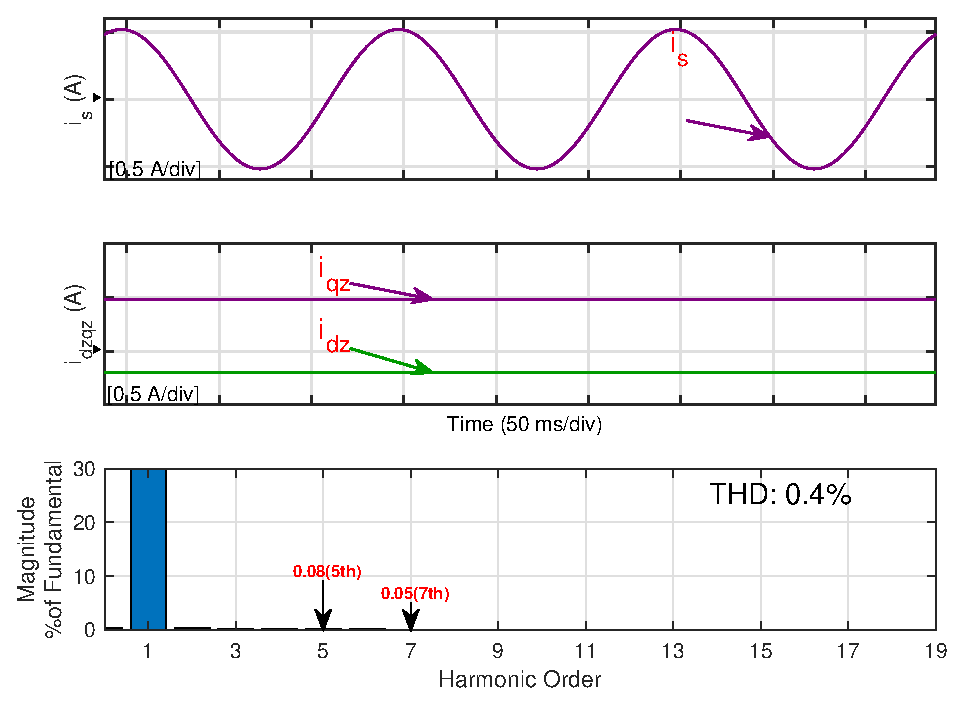
\includegraphics[width=\linewidth]{./MPCMidSpeedLowLoadSteadyState}
    \caption{Low load: \(T=0.3~\mathrm{N\,m}\),\\ THD \(=0.4\%\).}
    \label{fig:M2PCIdeal_1000rpm_low}
  \end{subfigure}\hfill
  % --- (b) Medium load ---
  \begin{subfigure}{0.485\textwidth}
    \centering
    % Replace with your exported plot/image
    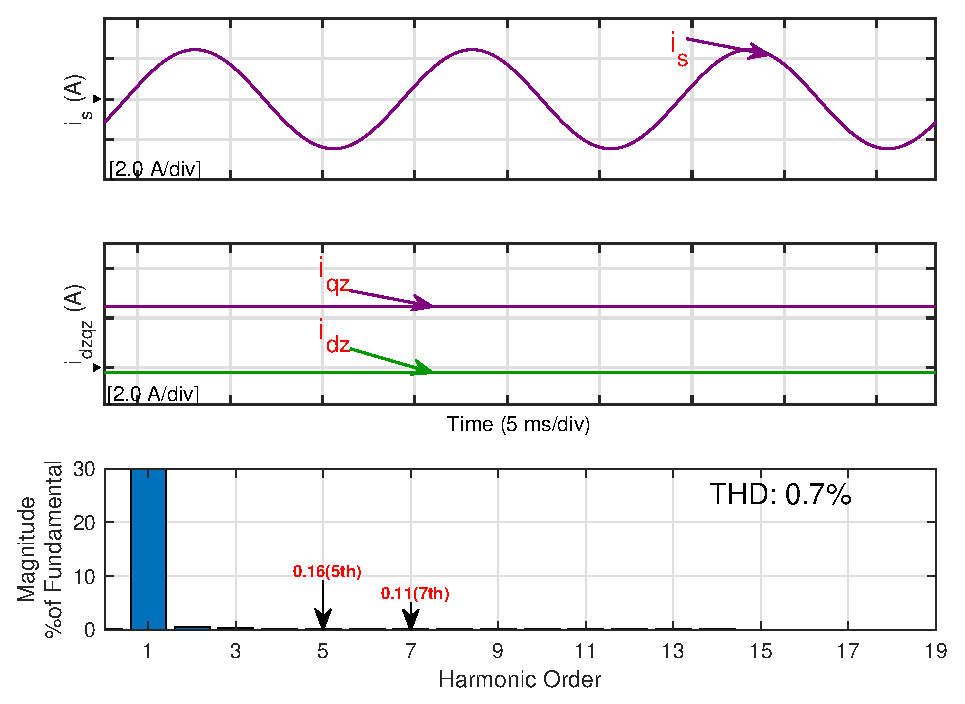
\includegraphics[width=\linewidth]{./MPCMidSpeedMidLoadSteadyState}
    \caption{Medium load: \(T=1.75~\mathrm{N\,m}\),\\ THD \(=0.7\%\).}
    \label{fig:M2PCIdeal_1000rpm_med}
  \end{subfigure}

  \caption{Modulated MPC (SVM-based) steady state at 50\% rated speed (1000 rpm, ideal model). Each panel shows phase currents, \(i_{dq}\), and THD. The modulated formulation yields very low harmonic content at both loads.}
  \label{fig:M2PCIdeal_1000rpm}
\end{figure}

\subsubsection{Low Speed Operation}
Under an ideal plant/inverter (no non-linearities or disturbances), the modulated MPC maintains accurate sensorless control at very low speeds. At 5\% rated (100~rpm), the phase-current THD is 0.3\% at low load (\(0.3~\mathrm{N\,m}\), see Fig.~\ref{fig:M2PCIdeal_100rpm_low}) and 0.4\% at rated load (\(3.5~\mathrm{N\,m}\), see Fig.~\ref{fig:M2PCIdeal_100rpm_high}); at 10\% rated (200~rpm), the THD is 0.5\% at low load (\(0.3~\mathrm{N\,m}\), see Fig.~\ref{fig:M2PCIdeal_200rpm_low}) and 0.1\% at rated load (\(3.5~\mathrm{N\,m}\), see Fig.~\ref{fig:M2PCIdeal_200rpm_high}). Across these cases the controller tracks with negligible steady-state error and fixed-frequency, SVM-based actuation that suppresses staircase ripple. Overall, the low-speed THD is comparable to or better than the PI baseline and far below FCS, evidencing robust performance under all tested loads in the absence of disturbances.
% Requires in preamble:
% \usepackage{graphicx}
% \usepackage{subcaption}

% ---------- MPC at 5% rated (100 rpm) ----------
\begin{figure}[t]
  \centering
  % Low load
  \begin{subfigure}{0.485\textwidth}
    \centering
    % Replace with your exported plot/image
    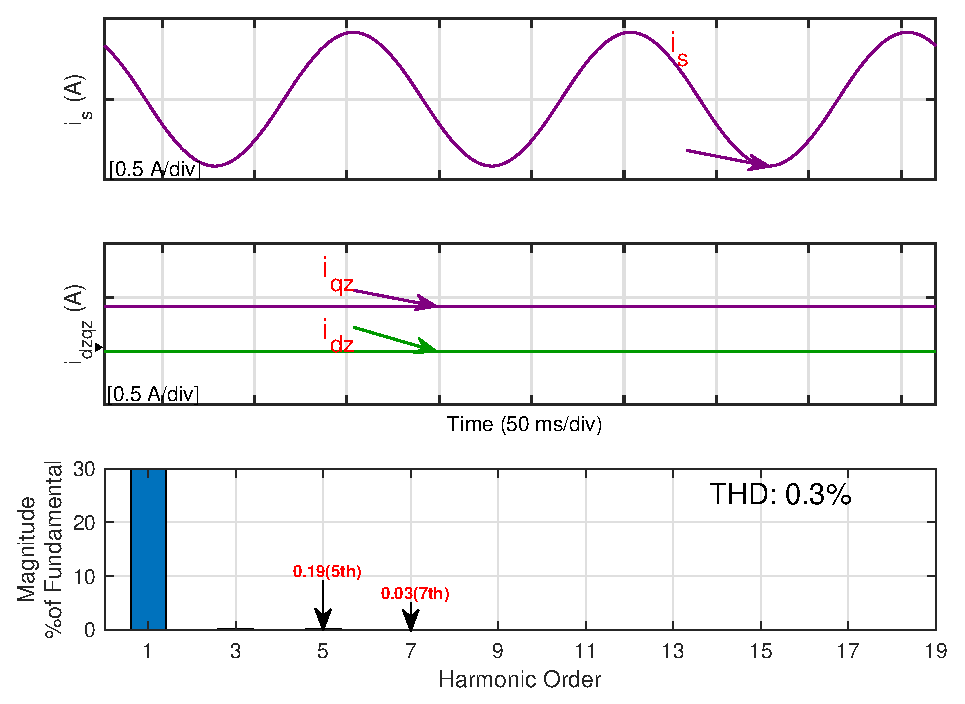
\includegraphics[width=\linewidth]{./MPCSteadyStateLowLoad100Rpm}
    \caption{Low load: \(T=0.3~\mathrm{N\,m}\); THD \(=0.3\%\).}
    \label{fig:M2PCIdeal_100rpm_low}
  \end{subfigure}\hfill
  % Rated load
  \begin{subfigure}{0.485\textwidth}
    \centering
    % Replace with your exported plot/image
    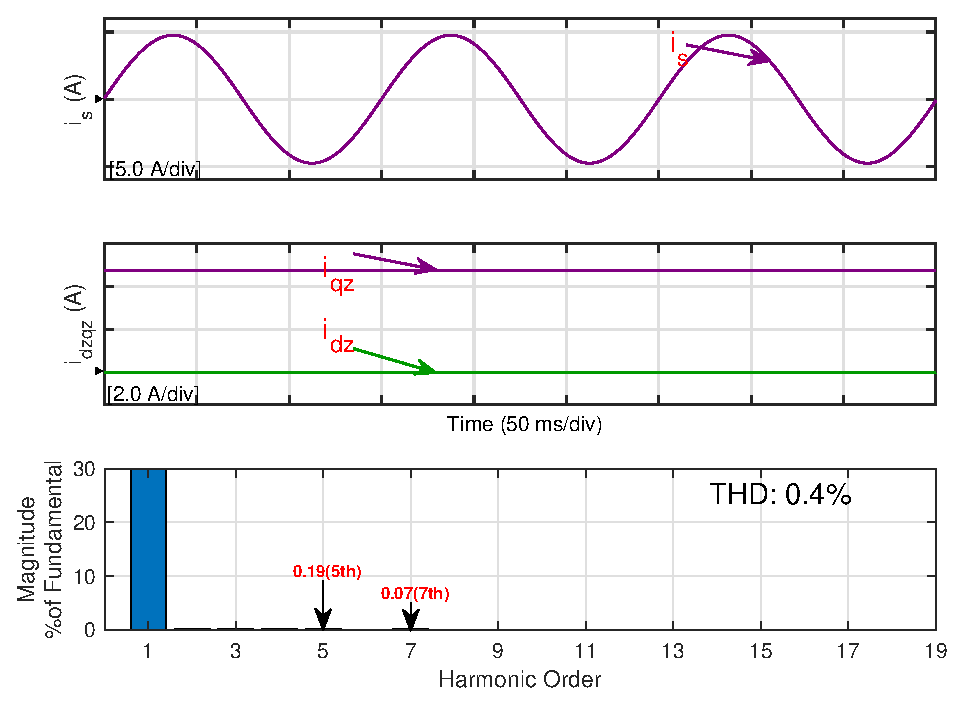
\includegraphics[width=\linewidth]{./MPCSteadyStateHighLoad100Rpm}
    \caption{Rated load: \(T=3.5~\mathrm{N\,m}\); THD \(=0.4\%\).}
    \label{fig:M2PCIdeal_100rpm_high}
  \end{subfigure}
  \caption{Modulated MPC (SVM-based) at 5\% rated speed (100 rpm, ideal model). Each panel shows phase currents, \(i_{dq}\), and THD.}
  \label{fig:M2PCIdeal_100rpm}
\end{figure}

% ---------- MPC at 10% rated (200 rpm) ----------
\begin{figure}[t]
  \centering
  % Low load
  \begin{subfigure}{0.485\textwidth}
    \centering
    % Replace with your exported plot/image
    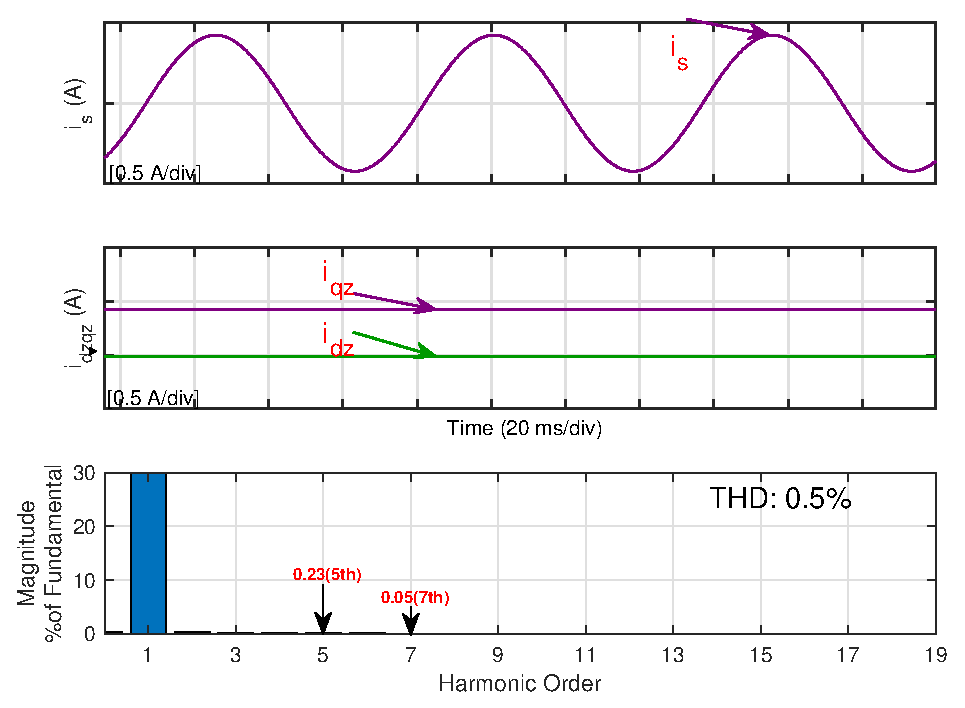
\includegraphics[width=\linewidth]{./MPCSteadyStateLowLoad200Rpm}
    \caption{Low load: \(T=0.3~\mathrm{N\,m}\); THD \(=0.5\%\).}
    \label{fig:M2PCIdeal_200rpm_low}
  \end{subfigure}\hfill
  % Rated load
  \begin{subfigure}{0.485\textwidth}
    \centering
    % Replace with your exported plot/image
    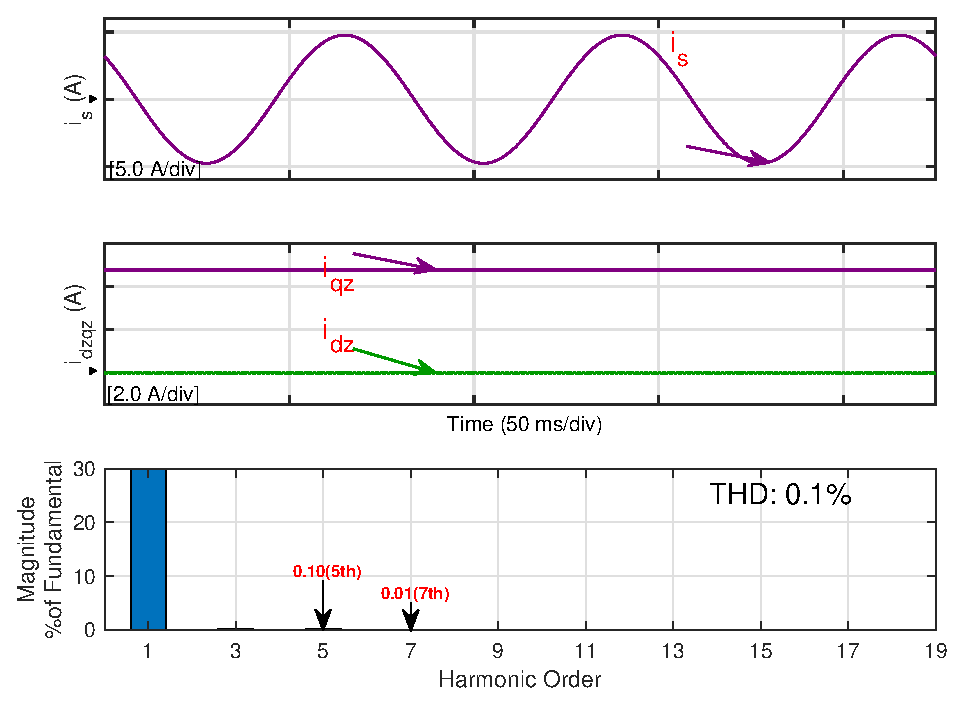
\includegraphics[width=\linewidth]{./MPCSteadyStateHighLoad200Rpm}
    \caption{Rated load: \(T=3.5~\mathrm{N\,m}\); THD \(=0.1\%\).}
    \label{fig:M2PCIdeal_200rpm_high}
  \end{subfigure}
  \caption{Modulated MPC (SVM-based) at 10\% rated speed (200 rpm, ideal model). Each panel shows phase currents, \(i_{dq}\), and THD.}
  \label{fig:M2PCIdeal_200rpm}
\end{figure}

\subsubsection{Dynamic Performance}
With an ideal plant/inverter (no non-linearities or disturbances), the modulated MPC tracks speed commands within the 10–50\% band (100~rpm \(\rightarrow\) 1000~rpm) cleanly at both load extremes. At \emph{low load} (10\% rated, \(0.3~\mathrm{N\,m}\)), Fig.~\ref{fig:M2PCDyn_100to1000_low} shows overshoot \(\mathbf{<10\%}\) and negligible steady-state error; at rated load (\(3.5~\mathrm{N\,m}\)), Fig.~\ref{fig:M2PCDyn_100to1000_rated} exhibits similarly well-damped behavior with a modestly slower rise. In both cases, the SVM-realized average voltage yields markedly smoother \(i_q\)/phase currents—far lower torque ripple than FCS and noticeably lower than PI—confirming robust dynamic performance across the tested range.
% Requires in preamble:
% \usepackage{graphicx}
% \usepackage{subcaption}

\begin{figure}[t]
  \centering
  % --- (a) Low load ---
  \begin{subfigure}{0.485\textwidth}
    \centering
    % Replace with your exported plot/image
    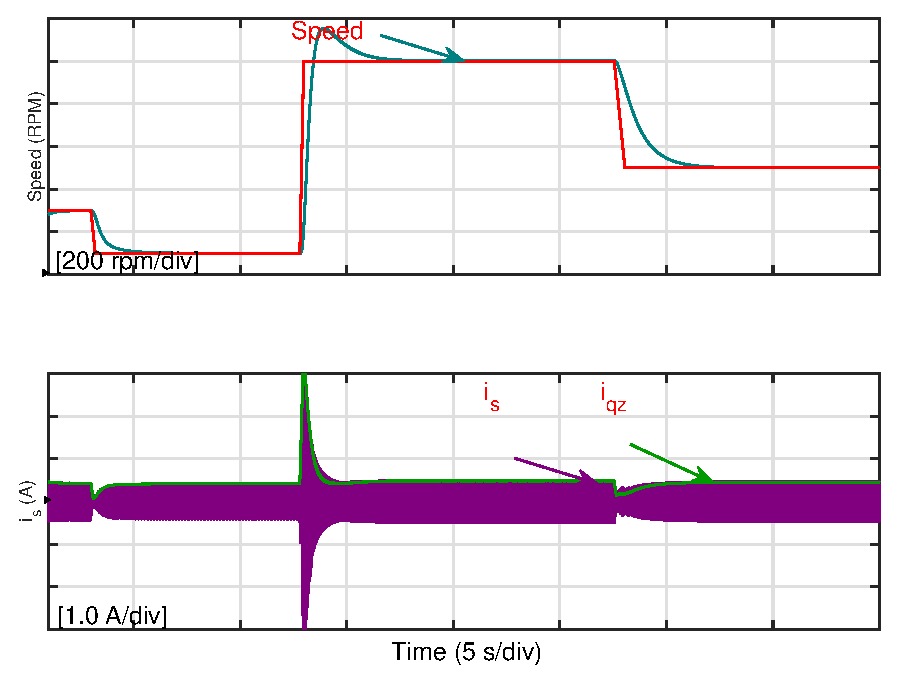
\includegraphics[width=\linewidth]{./MPCDynamicResponseLowLoad}
    \caption{Low load: \(T=0.3~\mathrm{N\,m}\). Overshoot \(<10\%\); negligible steady-state error; smooth \(i_q\)/phase currents.}
    \label{fig:M2PCDyn_100to1000_low}
  \end{subfigure}\hfill
  % --- (b) Rated load ---
  \begin{subfigure}{0.485\textwidth}
    \centering
    % Replace with your exported plot/image
    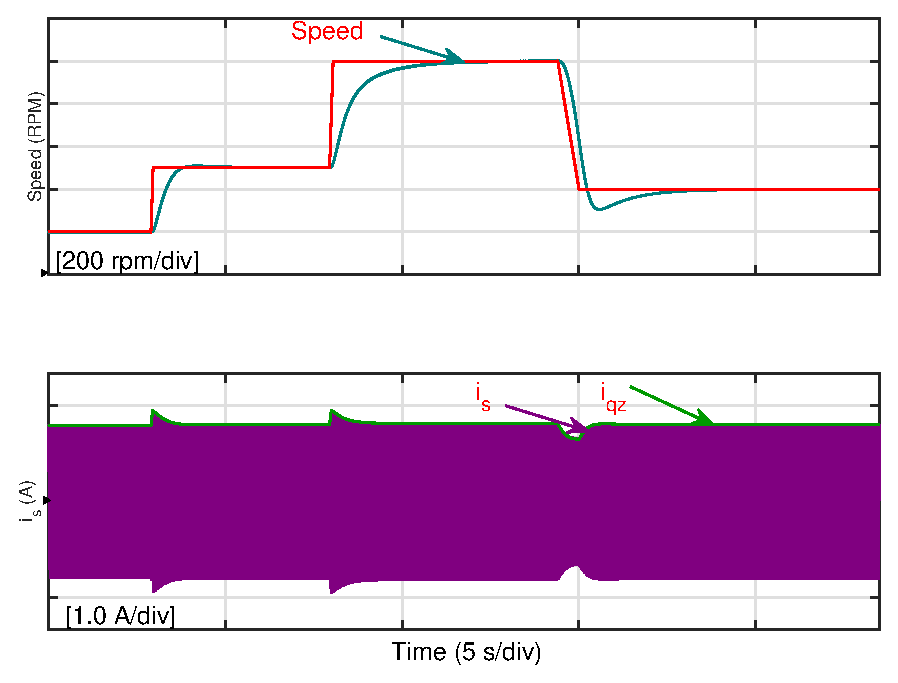
\includegraphics[width=\linewidth]{./MPCDynamicResponseHighLoad}
    \caption{Rated load: \(T=3.5~\mathrm{N\,m}\). Overshoot \(<10\%\); slightly slower rise; very low torque ripple.}
    \label{fig:M2PCDyn_100to1000_rated}
  \end{subfigure}

  \caption{Modulated MPC (SVM-based) dynamic response (ideal model) for speed changes within the \(10\%\!\to\!50\%\) rated band (100~rpm to 1000~rpm). Each panel shows command vs.\ speed, \(i_q\), and phase currents. The modulated formulation yields markedly smoother currents and lower torque ripple than FCS and PI.}
  \label{fig:M2PCDyn_100to1000}
\end{figure}

\subsubsection{Parameter Variation}
At 5\% rated speed (100~rpm), using a biased prediction model (\(R_s{+}25\%\), \(L_{d,q}{-}25\%\)) leaves the modulated MPC’s steady-state quality unchanged: phase-current THD stays at 0.3\% (Fig.~\ref{fig:M2PCParamVariation}). The fixed-frequency, SVM-based actuation and per-sample voltage optimization make the controller largely insensitive to moderate \(R\!-\!L\) errors—more robust than PI (1.3\% \(\rightarrow\) 1.7\%) and far better than FCS (32\% \(\rightarrow\) 41\%).

% Requires in preamble:
% \usepackage{graphicx}

\begin{figure}[H]
  \centering
  % Replace with your exported composite plot (speed, dq currents, phase currents, THD)
  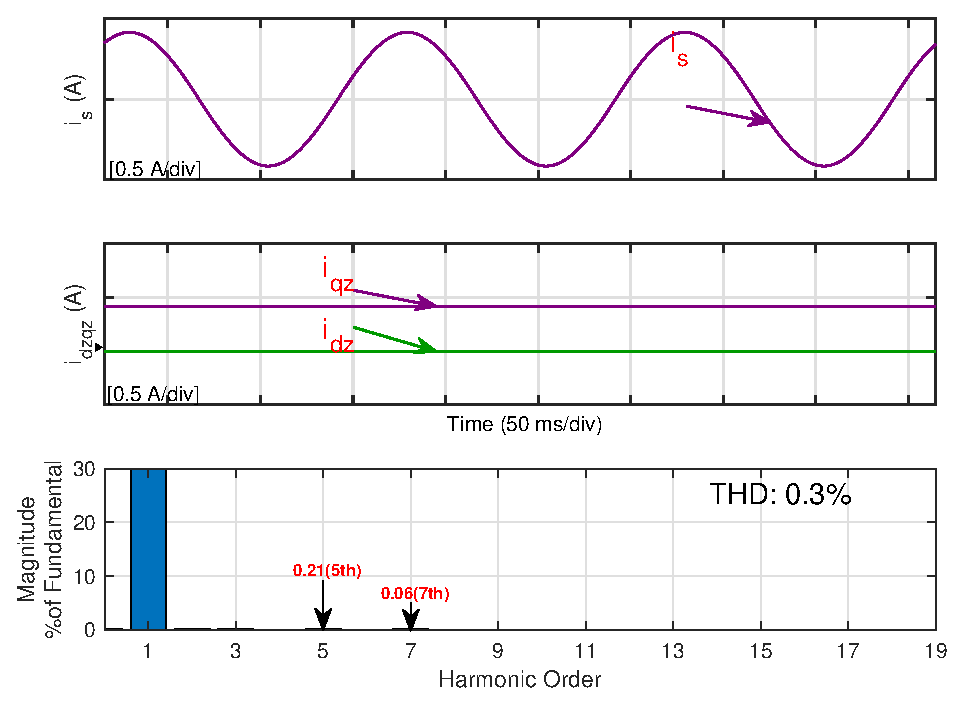
\includegraphics[width=0.6\linewidth]{./MPCParameterVariation}
  \caption{Modulated MPC under parameter variation at 5\% rated speed (100 rpm, ideal model).
  The prediction model uses \(R_s{+}25\%\) and \(L_{d,q}{-}25\%\). The figure reports  phase currents, \(d\)- and \(q\)-axis currents, and the THD comparison, which remains at \(\mathbf{0.3\%}\)—indistinguishable from the no-variation case—indicating high robustness of bandwidth/cutoff and harmonic performance.}
  \label{fig:M2PCParamVariation}
\end{figure}

\subsubsection{Load Variation}
At 1000 rpm the load torque was stepped from 10\% to 100\% of rated in 20\% increments, each held to steady state. As shown in Fig.~\ref{fig:M2PCLoadVariation}, the modulated MPC maintains the commanded speed without droop; \(i_q\) increases in clean, proportional steps to furnish the added torque, and the phase currents remain smooth thanks to the fixed-frequency SVM realization of the optimized average voltage. Transients are well damped and steady-state ripple stays low throughout, evidencing robust disturbance rejection under load changes.
% Requires in preamble:
% \usepackage{graphicx}

\begin{figure}[H]
  \centering
  % Replace with your exported composite plot that contains
  % (left) speed response, (middle) dq-currents, (right) phase currents
  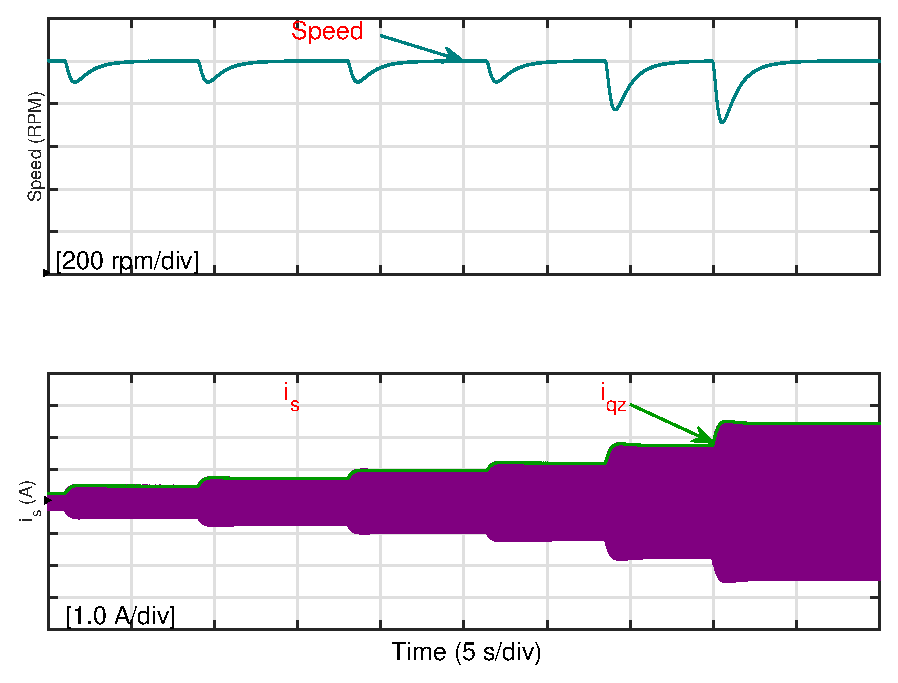
\includegraphics[width=0.6\linewidth]{./MPCLoadVariation}
  \caption{Modulated MPC under load variation at 50\% rated speed (1000 rpm, ideal model).
  The composite figure shows motor speed, \(q\)-axis currents, and phase currents during torque steps from 10\% to 100\% of rated in 20\% increments.}
  \label{fig:M2PCLoadVariation}
\end{figure}

% bridge to proposed controller
